\documentclass[pdf]
{beamer}
\usetheme{Copenhagen}


 \usecolortheme{rose}
% \useinnertheme[shadow]{rounded}
% \usecolortheme{dolphin}
 \useoutertheme{infolines}


\usepackage[spanish]{babel}
\usepackage{lmodern}
\usepackage{color}

\newcommand{\automation}{\textit{Automatizaci\'on}}
\newcommand{\tdd}{\textit{TDD}}
\newcommand{\testing}{\textit{testing}}
\newcommand{\android}{\textit{Android}}
\newcommand{\espresso}{\textit{Espresso}}


\newcommand{\myitem}[1]% #1 = text inside bullet
{
  \par\vspace{3pt}\hspace*{3pt}%
  \begin{pgfpicture}{-1ex}{-0.65ex}{1ex}{1ex}
    \usebeamercolor[fg]{item projected}
    {\pgftransformscale{1.75}\pgftext{\normalsize\pgfuseshading{bigsphere}}}
    {\pgftransformshift{\pgfpoint{0pt}{0.5pt}}
      \pgftext{\usebeamerfont*{item projected}#1}}
  \end{pgfpicture}%
  \hspace{1pt}%
}

\mode<presentation>{}

\title{Automatizaci\'on de pruebas en \android{}}
\subtitle{usando \textit{Espresso}}
\author{Jorge Bautista\\jorge.bautista@globant.com}


\AtBeginSection[]
{
\begin{frame}
    \frametitle{Contenido}
    \tableofcontents[currentsection]
\end{frame}
}


\AtBeginSubsection[]
{
\begin{frame}
    \frametitle{Contenido}
    \tableofcontents[currentsection,currentsubsection]
\end{frame}
}

% To define Globant's green
% \definecolor{GlobantGreen}{RGB}{193,216,47}
% \setbeamercolor{structure}{fg=GlobantGreen}

\begin{document}

%Trying to ADD Globant images to the template 
%     \addtobeamertemplate{frametitle}{}{%
%       \begin{textblock*}{100mm}(.85\textwidth,-1cm)
%       
\includegraphics[height=1cm,width=2cm]{figures/globant}
%       \end{textblock*}
%     }
     
    \begin{frame}
        \titlepage
    \end{frame}


    \section{Automatizaci\'on de pruebas}


        \subsection{Pruebas de regresi\'on}
        \begin{frame}{Pruebas de regresi\'on}
	  Probar toda la aplicaci\'on en busca de posibles errores derivados de la modificaci\'on de un m\'odulo o funcionalidad . Se requiere de un gran trabajo para poder validar la funcionalidad de todo el sistema.
        \end{frame}
        
        \subsection{Automatizaci\'on}
        \begin{frame}{?`Qu\'e es Automatizaci\'on?}

	      Permiten la ejecuci\'on r\'apida de una serie de pruebas de regresi\'on con el objetivo de verificar una y otra vez que una modificaci\'on en el c\'odigo no ha generado nuevos errores en la aplicaci\'on.
	      
	      \begin{block}<2->{Meta principal}
		\textbf{Incrementar periodicidad y facilitar el \textit{testing}} 
	      \end{block}

        \end{frame}
        
        \subsection{Importancia de la automatizaci\'on}
        \begin{frame}{Importancia de la automatizaci\'on}
            \begin{itemize}
             \item<2-> Valida que producto haga lo que la especificaci\'on dicta
             \item<3-> Funciona como documentaci\'on ya que es una muestra ``viva''
             \item<4-> Evita ambig\"uedades en la comprensi\'on del requerimiento. Hay un feedback m\'as r\'apido por parte del cliente.
             \item<5-> Permite a testers y desarrolladores enfocarse en lo importante
             \item<6-> Aumenta la confianza entre testers y desarrolladores
             \item<7-> Facilita el mantenimiento
		\begin{itemize}
		  \item<8-> Es f\'acil saber lo que hace una pieza de software
		  \item<9-> Nueva versi\'on del SDK de Android
		  \item<10-> Despu\'es de un cambio en el c\'odigo; modificaciones sin riesgo (``red de seguridad'' contra regresiones)
		\end{itemize}

            \end{itemize}

        \end{frame}
	
	\subsection{Recomendaciones}   

	\begin{frame}{Recomendaciones para el dise\~no de pruebas automatizadas}
	  \begin{itemize}
	    \item<2-> Uso de bater\'ia
	    \item<3-> Rendimiento de la aplicaci\'on (con historial de m\'etricas)
	    \item<4-> Consumo de datos m\'oviles
	    \item<5-> Contextos exceptionales: red, almacenamiento
	    \item<6-> Evita acoplar datos est\'aticos + \textit{Data Fuzzing}
	    \item<7-> No automatices todo. Considera mantenimiento, complejidad y falso sentido de seguridad. 
	    \item<8-> Trabajar en equipo con los testers
	    \item<9-> Al alcance de todos \& Lejos de tu m\'aquina local
	    \item<10-> El tiempo de ejecuci\'on de las pruebas es importante, encuentra la forma de acortarlo

	  \end{itemize}

	\end{frame}
        
    
    \section{Automatizaci\'on con Espresso}
    \subsection{Tecnolog\'ias de automatizaci\'on}
    \begin{frame}{Algunas de tecnolog\'ias de automatizaci\'on}
        \begin{block}<2->{Web}
	    Selenium, Watir, Windmill, \textbf{Ranorex}, Sahi, Tellurium 
	\end{block}
	\begin{block}<3->{Escritorio}
	    Squish, \textbf{Ranorex}, TestComplete, Test Studio, eggPlant
	\end{block}
	\begin{block}<4->{M\'ovil}
	    Appium, Selendroid, Robotium, MonkeyRunner, \textbf{Ranorex}, DeviceAnywhere, eggPlant, SilkMobile, SeeTest, MonkeyTalk, Espresso
	\end{block}

    \end{frame}
    
    \subsection{?`Qu\'e es Espresso?}
   
    \subsubsection{Definici\'on}
    \begin{frame}{Definici\'on}
	Es un framework para realizar pruebas de UI en aplicaciones Android que se desarroll\'o sobre tecnolog\'ias como \textit{Instrumentation} y \textit{Hamcrest}
	
	\begin{block}<2->{?`Porque usarlo?}
	
	  \begin{itemize}
	    \item <3-> Google lo usa
	    \item <4-> F\'acil de usar
	    \item <5-> Sintaxis declarativa, limpia e intuitiva
	    \item <6-> Velocidad
	    \item <7-> \textit{Default Async Thread Pool} (incronizaci\'on)
	  \end{itemize}
	  
	\end{block}

    \end{frame}

    \subsubsection{Componentes de Espresso y c\'omo se usan}
    \begin{frame}[t]{Componentes de Espresso y c\'omo se usan}
    
      \begin{columns}
        \column{0.5\textwidth}
        \begin{enumerate}
         \item Se busca el elemento con un \textbf{\textit{ViewMatcher}}
         \item Se interactua con el elemento con un \textbf{\textit{ViewAction}}
         \item Se verifica que la vista reaccione correctamente con un \textbf{\textit{ViewAssertion}}
        \end{enumerate}
	\column{0.5\textwidth}
	\begin{block}<2->{Matchers (encuentran elementos)}
	withText, withId, withInputType, withTagValue, isChecked, isClickable, isEnabled, etc.
	\end{block}
	\begin{block}<3->{Actions (accionan elementos)}
	click, doubleClick, longClick, clearText, pressKey, scrollTo, swipeDown, swipeLeft, swipeRight, swipeUp, typeText, etc.
	\end{block}
	\begin{block}<4->{Assertions (verifican estado de vista)}
	doesNotExist, matches, selectedDescendantsMatch
	\end{block}
      \end{columns}
  
    \end{frame}

    
    \subsection{?`C\'omo integrar Espresso?}
    \begin{frame}{Integraci\'on}
    
      \begin{columns}
	\column{0.5\textwidth}
	  \begin{block}<2->{\myitem{1} Android Support Repository}
	    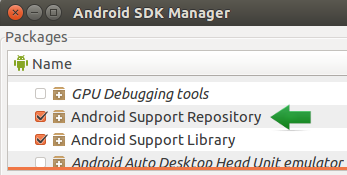
\includegraphics[scale=.4]{figures/integration_steps/step_1}
	  \end{block}
	\column{0.5\textwidth}
	  \begin{block}<3->{\myitem{2} Definir Test Runner}
	  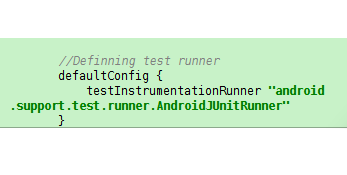
\includegraphics[scale=.4]{figures/integration_steps/step_2}
	  \end{block}       
      \end{columns}

      \begin{block}<4->{\myitem{3} Agregar dependencias}
	  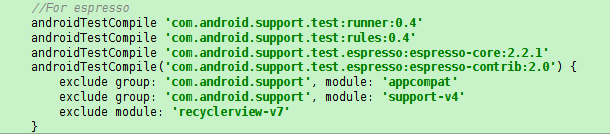
\includegraphics[scale=.4]{figures/integration_steps/step_3}
      \end{block}       
  
       
        
        
        
    \end{frame}

    \section{Demo}
    \begin{frame}
      \begin{center}
      \Huge{Demo}
      \end{center}
    \end{frame}

    

    
    \section{Bibliograf\'ia}
    \begin{frame}{Bibliograf\'ia (1/3)}
      \frametitle<presentation>{Bibliograf\'ia (1/3)}
      
      \begin{thebibliography}{10}    

      \beamertemplatebookbibitems
	\bibitem{Specification by Example}
	  Gojko Adzic, {\em Specification by Example}
	  \newblock Manning Publications, 2011
      \setbeamertemplate{bibliography item}[online]
	\bibitem{InfoQ}
	  InfoQ, {\em Thoughts on Test Automation in Agile}
	  \newblock \small{\href{http://www.infoq.com/articles/thoughts-on-test-automation-in-agile}{http://www.infoq.com/articles/thoughts-on-test-automation-in-agile}}
      \setbeamertemplate{bibliography item}[online]
	\bibitem{WikipediA}
	  WikipediA, {\em Software testing}
	  \newblock \href{https://en.wikipedia.org/wiki/Software\_testing}{https://en.wikipedia.org/wiki/Software\_testing}
	  
      \setbeamertemplate{bibliography item}[online]
	\bibitem{ApplicationTypes}
	  J.D. Meier's Blog, {\em Application Types (App Types) - The Early Years}
	  \newblock {\tiny \href{http://blogs.msdn.com/b/jmeier/archive/2010/07/29/application-types-app-types-the-early-years.aspx}{http://blogs.msdn.com/b/jmeier/archive/2010/07/29/application-types-app-types-the-early-years.aspx}}
      
      \setbeamertemplate{bibliography item}[online]
	\bibitem{AutomationTools}
	  Software Testing Tools, {\em Software Test Automation Tools}
	  \newblock {\small \href{http://www.testingtools.com/test-automation/}{http://www.testingtools.com/test-automation/}}
      

      \setbeamertemplate{bibliography item}[online]
	\bibitem{Voguella}
	  Voguella, {\em Android user interface testing with Espresso}
	  \newblock {\small\href{http://www.vogella.com/tutorials/AndroidTestingEspresso/article.html}{http://www.vogella.com/tutorials/AndroidTestingEspresso/article.html}}
	  
      \end{thebibliography}
      
    \end{frame}
    
    \begin{frame}{Bibliograf\'ia (2/3)}
      \frametitle<presentation>{Bibliograf\'ia (2/3)}    
      
      
      \begin{thebibliography}{10}    
	  
      \setbeamertemplate{bibliography item}[online]
	\bibitem{Android Research Blog}
	  Android Research Blog, {\em Introduction to Android Espresso}
	  \newblock {\tiny\href{https://androidresearch.wordpress.com/2015/04/04/an-introduction-to-espresso/}{https://androidresearch.wordpress.com/2015/04/04/an-introduction-to-espresso/}}
	  
      \setbeamertemplate{bibliography item}[online]
	\bibitem{Developer Android}
	  Developer Android, {\em Testing Fundamentals}
	  \newblock {\small\href{http://developer.android.com/intl/es/tools/testing/testing\_android.html}{http://developer.android.com/intl/es/tools/testing/testing\_android.html}}
	  
      \setbeamertemplate{bibliography item}[online]
	\bibitem{Software Testing Help}
	  {\small Software Testing Help, {\em 5 Best Automation Tools for Testing Android Applications}}
	  
	  \newblock \tiny{\href{http://www.softwaretestinghelp.com/5-best-automation-tools-for-testing-android-applications/}{http://www.softwaretestinghelp.com/5-best-automation-tools-for-testing-android-applications/}}
	  
      \setbeamertemplate{bibliography item}[online]
	\bibitem{Software Testing Help}
	  \small{Software Testing Help, {\em Beginner's Guide to Mobile App Testing}}
	  \newblock {\tiny \href{http://www.softwaretestinghelp.com/beginners-guide-to-mobile-application-testing/}{http://www.softwaretestinghelp.com/beginners-guide-to-mobile-application-testing/}}

      \setbeamertemplate{bibliography item}[online]
	\bibitem{Stack Overflow}
	  Stack Overflow, {\em Gradle test command not running any tests}
	  \newblock {\small\href{http://stackoverflow.com/questions/31975388/}{http://stackoverflow.com/questions/31975388/}}

      \end{thebibliography}
      
      
      
      
    \end{frame}
    
    
    \begin{frame}{Bibliograf\'ia (3/3)}
      \frametitle<presentation>{Bibliograf\'ia (3/3)}    
      
      
      \begin{thebibliography}{10}    

    \setbeamertemplate{bibliography item}[online]
	\bibitem{Testing for Android}
	  YouTube, {\em Testing for Android}
	  \newblock {\small \href{https://www.youtube.com/watch?v=Od9l-OGAXC8}{https://www.youtube.com/watch?v=Od9l-OGAXC8}}

      \setbeamertemplate{bibliography item}[online]
	\bibitem{AutomationTools}
	  YouTube, {\em GTAC 2013: Espresso: Fresh Start to Android UI Testing}
	  \newblock {\small \href{https://www.youtube.com/watch?v=T7ugmCuNxDU}{https://www.youtube.com/watch?v=T7ugmCuNxDU}}
	  
      \setbeamertemplate{bibliography item}[online]
	\bibitem{Espresso for Android - a Demo}
	  You Tube, {\em Espresso for Android - a Demo}
	  \newblock \href{https://www.youtube.com/watch?v=qtKx1WxK7cw}{https://www.youtube.com/watch?v=qtKx1WxK7cw}
	  
      \setbeamertemplate{bibliography item}[online]
	\bibitem{Large Espresso Example}
	  You Tube, {\em Android Testing - Getting Started with Espresso 2.0}
	  \newblock \href{https://www.youtube.com/watch?v=TGU0B4qRlHY}{https://www.youtube.com/watch?v=TGU0B4qRlHY}

      \end{thebibliography}
      
    \end{frame}
    
\end{document}